% Analisi dei requisiti

\chapter{Analisi dei requisiti}

% TODO: CTO e CEO in glossary?
% TODO: feature in glossary?
PastBot nasce da un insieme di nuove tecnologie e dalla necessità di ampliare i
metodi a disposizione per l'acquisito di prodotti da PastBook.
La prima attività del progetto è stata dunque la consultazione del parere del
servizio \textit{marketing} e del \gls{ceo} riguardo la creazione di un nuovo
modo per interagire con gli utenti. Dopo che la creazione di un \textit{bot}
per la piattaforma Facebook è stata accolta, si è passati a valutare l'opinione
di una parte dell'utenza di PastBook. L'utenza ascoltata fa parte del gruppo di
\textit{tester} di PastBook, che ha deciso di avere un accesso anticipato ai
nuovi prodotti in cambio di una loro valutazione. L'azienda si è rivolta a loro
anche per valutare l'interessamento nell'utilizzo di un futuro \textit{bot} per
Facebook, idea che è stata accolta favorevolmente in buona parte.

Si è quindi passati all'interazione con il reparto di codifica, che ha dovuto
eseguire un'analisi dei requisiti per estrapolare i casi d'uso prima di poter
cominciare a progettare il prodotto.

\newpage

\section{Requisiti di PastBot}

PastBot suddivide l'utenza in due categorie principali:
l'utenza non registrata, ovvero che non ha mai scritto al \textit{bot} e
l'utenza registrata, cioè che ha almeno una volta scritto al \textit{bot}.

\subsection{UC0: caso d'uso generale}
\label{uc:uc0}

\begin{itemize}
  \item \textbf{Attori}: Utente Non Autenticato, Utente Autenticato;
  \item \textbf{Descrizione}: un utente innanzitutto deve iniziare la
conversazione con il \textit{bot}. Dopo di che avrà a disposizione il sistema di
conversazione in cui poter mandare messaggi al \textit{bot};
  \item \textbf{Precondizione}: l'utente deve aver un account Messenger e deve
averci effettuato la connessione;
  \item \textbf{Postcondizione}: il sistema ha erogato le funzionalità
richieste dall'utente;
  \item \textbf{Flusso principale}:
  \begin{enumerate}
    \item L'Utente Non Autenticato può iniziare una conversazione per la prima
volta in assoluto (\hyperlink{UC1}{UC1})
    \item L'Utente Autenticato può inviare una richiesta di creare nuovo
album (\hyperlink{UC2}{UC2})
    \item L'Utente Autenticato può inviare una richiesta di visualizzare l'album
esistente (\hyperlink{UC3}{UC3})
    \item L'Utente Autenticato può inviare una richiesta riguardante le
informazioni sui costi (\hyperlink{UC4}{UC4})
    \item L'Utente Autenticato può inviare un comando per ricevere aiuto
(\hyperlink{UC5}{UC5})
    \item L'Utente Autenticato può inviare una richiesta di visualizzazione
dell'album nel sito web (\hyperlink{UC6}{UC6})
    \item L'Utente Autenticato può inviare un comando non valido
(\hyperlink{UC7}{UC7})
    \item L'Utente Autenticato può inviare uno \textit{sticker}
(\hyperlink{UC8}{UC8})
    \item L'Utente Autenticato può inviare un allegato (\hyperlink{UC9}{UC9})
    \item L'Utente Autenticato può visualizzare il menù permanente.
(\hyperlink{UC11}{UC11})
  \end{enumerate}
\end{itemize}


\begin{figure}[H]
  \centering
  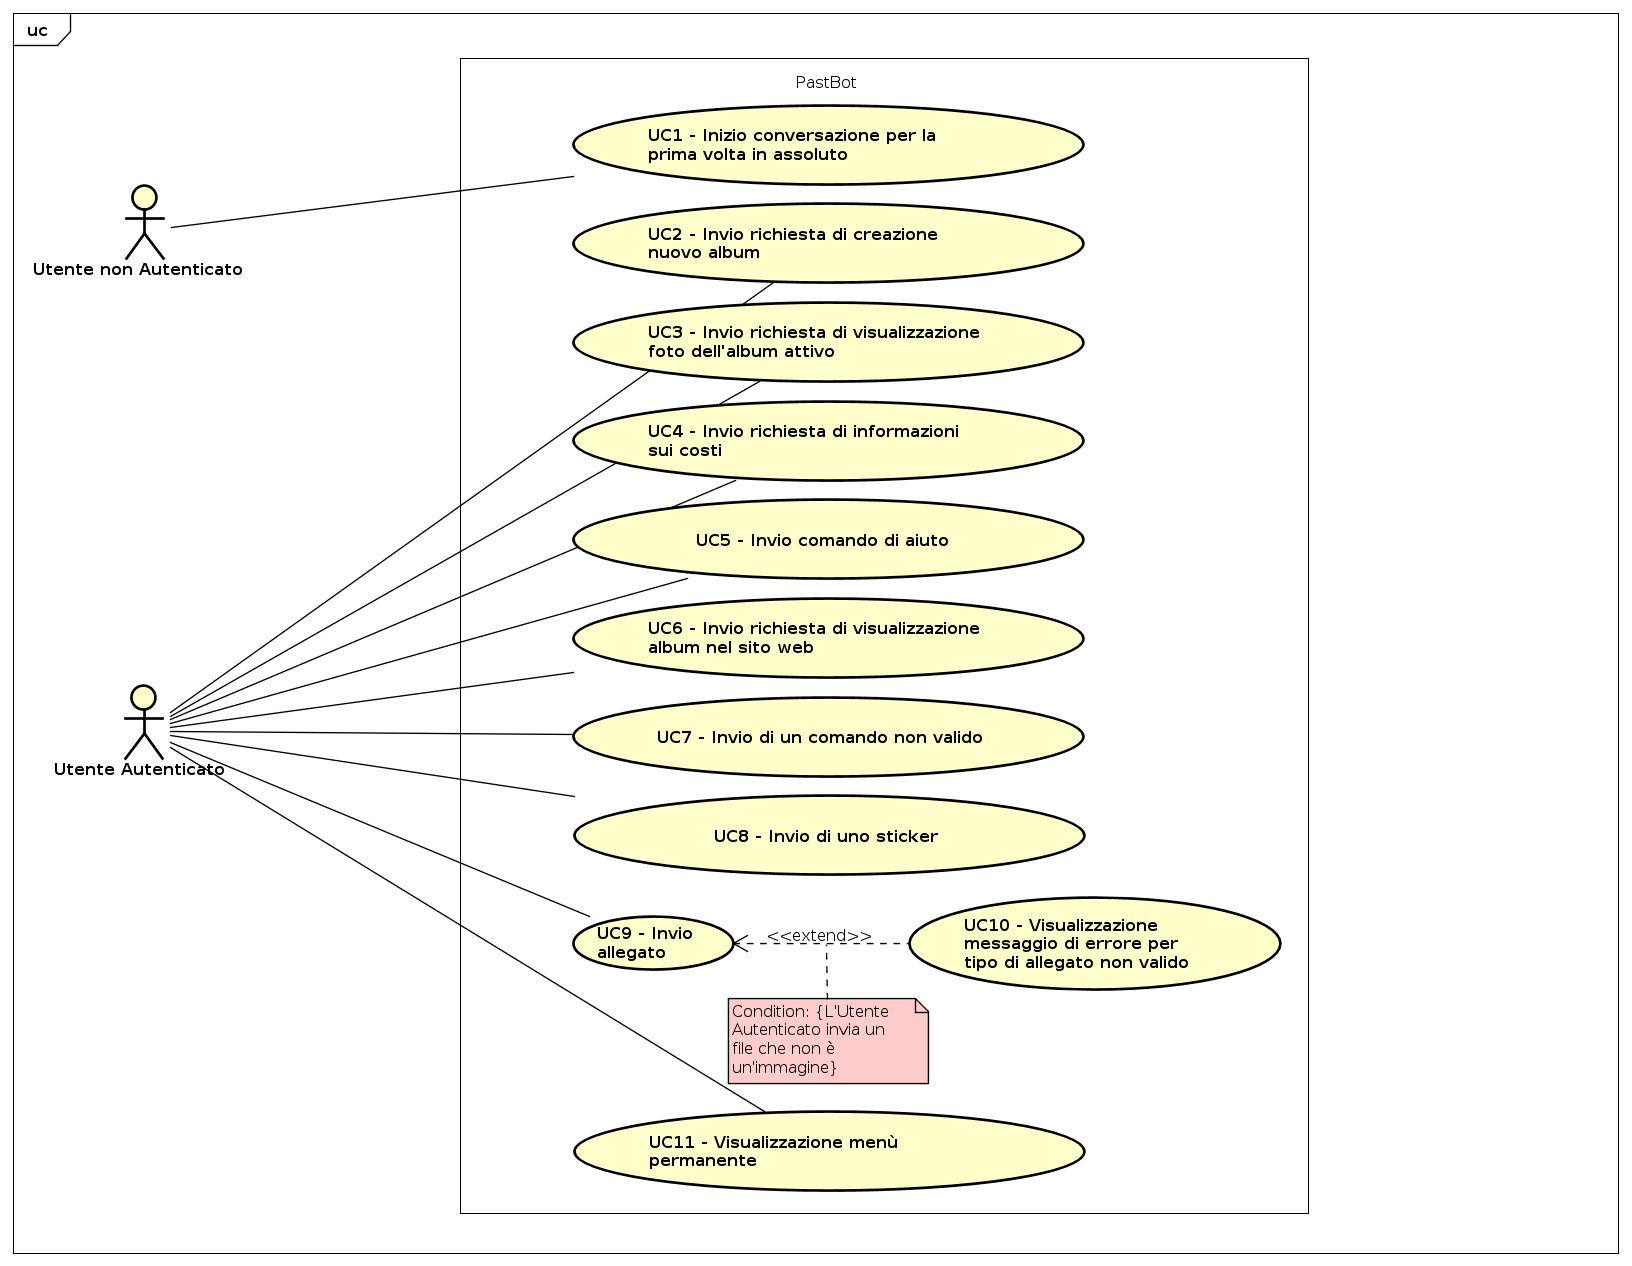
\includegraphics[scale=0.4]{useCase/UC0}
  \caption{UC0: caso d'uso generale}
\end{figure}


% \newpage

\subsection{UC1: inizio conversazione per la prima volta in assoluto}
\label{uc:uc1}
\hypertarget{UC1}{}

\begin{itemize}
  \item \textbf{Attori}: Utente Non Autenticato;
  \item \textbf{Descrizione}: l'Utente Non Autenticato vuole scrivere al
\textit{bot} per la prima volta in assoluto. Per fare questa azione dovrà
premere il bottone "Inizia" presente in Messenger;
  \item \textbf{Precondizione}: l'Utente Non Autenticato è iscritto alla
piattaforma di messaggistica Facebook Messenger;
  \item \textbf{Postcondizione}: l'Utente Non Autenticato ha inviato con
successo il suo primo messaggio al \textit{bot};
  \item \textbf{Flusso principale}:
  \begin{enumerate}
    \item L'Utente Non Autenticato clicca sul bottone apposito per iniziare la
conversazione
  \end{enumerate}
\end{itemize}



%%% INIZIO SEZIONE USE CASE 2 %%%
%\newpage

\subsection{UC2: invio richiesta di creazione di un nuovo album}
\label{uc:uc2}
\hypertarget{UC2}{}

\begin{itemize}
  \item \textbf{Attori}: Utente Autenticato;
  \item \textbf{Descrizione}: l'Utente Autenticato procede alla richiesta di
creazione di un nuovo album di foto. Gli verrà posta una domanda per avere
conferma della creazione, alla quale potrà rispondere in maniera affermativa o
negativa;
  \item \textbf{Precondizione}: l'Utente Autenticato ha cominciato la
conversazione con il \textit{bot};
  \item \textbf{Postcondizione}: l'Utente Autenticato ha gestito con successo
il proprio album;
  \item \textbf{Flusso principale}:
  \begin{enumerate}
    \item L'Utente Autenticato può confermare la creazione di un nuovo album
(\hyperlink{UC2.1}{UC2.1})
    \item L'Utente Autenticato può non confermare la creazione di un nuovo album
(\hyperlink{UC2.2}{UC2.2})
  \end{enumerate}
\end{itemize}

\begin{figure}[H]
  \centering
  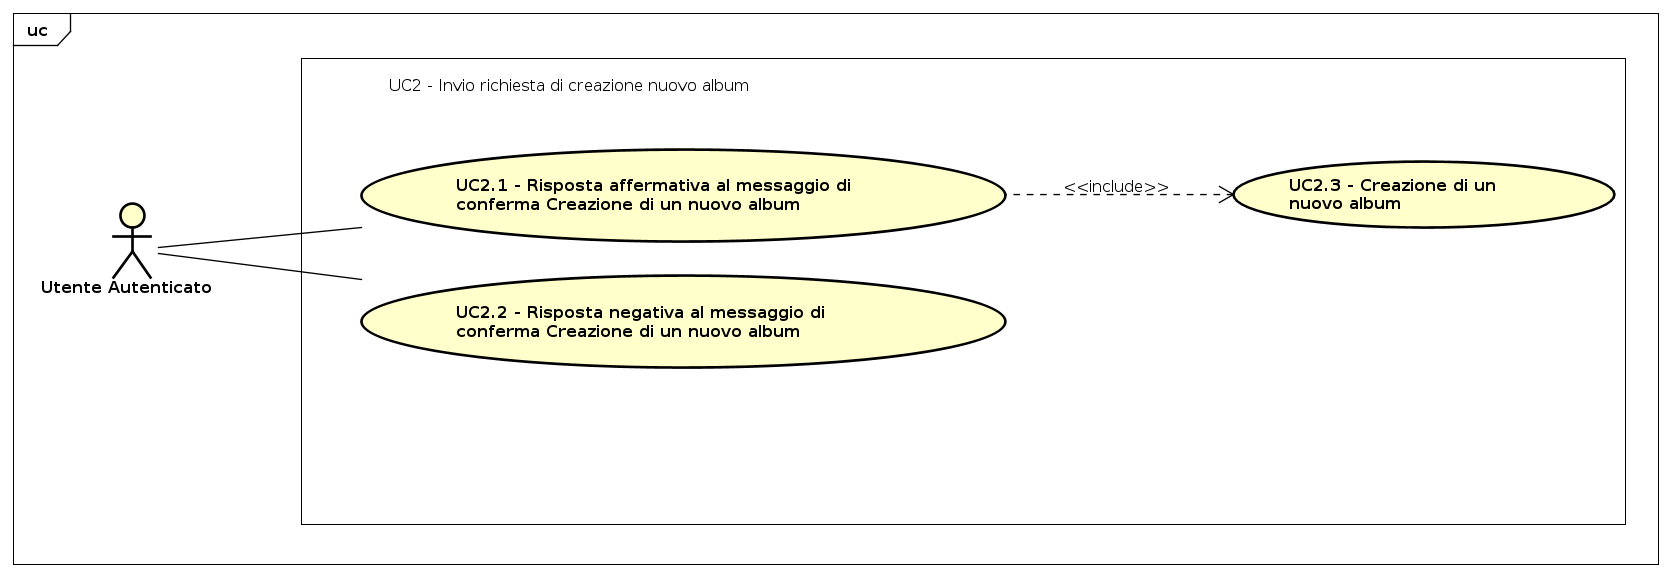
\includegraphics[scale=0.3]{useCase/UC2}
  \caption{UC2: invio richiesta di creazione di un nuovo album}
\end{figure}

%\newpage

\subsection{UC2.1: risposta affermativa al messaggio di conferma Creazione
nuovo album}
\label{uc:uc2.1}
\hypertarget{UC2.1}{}

\begin{itemize}
  \item \textbf{Attori}: Utente Autenticato;
  \item \textbf{Descrizione}: l'Utente Autenticato conferma la decisione di
voler creare un nuovo album;
  \item \textbf{Precondizione}: l'Utente Autenticato ha richiesto la creazione
di un nuovo album;
  \item \textbf{Postcondizione}: l'Utente Autenticato ha confermato con
successo la volontà di creare un nuovo album;
  \item \textbf{Flusso principale}:
  \begin{enumerate}
    \item L'Utente Autenticato conferma positivamente la creazione di un nuovo
album
  \end{enumerate}
\end{itemize}


%\newpage

\subsection{UC2.2: risposta negativa al messaggio di conferma Creazione nuovo
album}
\label{uc:uc2.2}
\hypertarget{UC2.2}{}

\begin{itemize}
  \item \textbf{Attori}: Utente Autenticato;
  \item \textbf{Descrizione}: l'Utente Autenticato decide di non voler più
creare un nuovo album;
  \item \textbf{Precondizione}: l'Utente Autenticato ha richiesto la creazione
di un nuovo album;
  \item \textbf{Postcondizione}: l'Utente Autenticato ha confermato con
successo la volontà di non procedere alla creazione di un nuovo album;
  \item \textbf{Flusso principale}:
  \begin{enumerate}
    \item L'Utente Autenticato conferma negativamente la creazione di un nuovo
album
  \end{enumerate}
\end{itemize}


%\newpage

\subsection{UC2.3: creazione di un nuovo album}
\label{uc:uc2.3}
\hypertarget{UC2.3}{}

\begin{itemize}
  \item \textbf{Attori}: Utente Autenticato;
  \item \textbf{Descrizione}: si ottiene un nuovo album vuoto in cui sarà
possibile inserire nuove foto;
  \item \textbf{Precondizione}: l'Utente Autenticato ha confermato
positivamente la volontà di creare un nuovo album;
  \item \textbf{Postcondizione}: l'Utente Autenticato dispone di un nuovo album;
  \item \textbf{Flusso principale}:
  \begin{enumerate}
    \item L'Utente Autenticato ha confermato positivamente la creazione di un
nuovo album
  \end{enumerate}
\end{itemize}


%%% FINE SEZIONE USE CASE 2 %%%

%%% INIZIO SEZIONE USE CASE 3 %%%
\newpage

\subsection{UC3: invio richiesta di visualizzazione foto dell'album attivo}
\label{uc:uc3}
\hypertarget{UC3}{}

\begin{itemize}
  \item \textbf{Attori}: Utente Autenticato;
  \item \textbf{Descrizione}: l'Utente può richiedere la visualizzazione della
lista delle foto attualmente caricate, su cui può decidere di cancellarne
alcune, di visualizzarle senza perdita di risoluzione o di acquistarle in un
album;
  \item \textbf{Precondizione}: l'Utente Autenticato ha cominciato la
conversazione con il \textit{bot};
  \item \textbf{Postcondizione}: l'Utente Autenticato ha visualizzato con
successo la lista delle foto presenti nel proprio album;
  \item \textbf{Flusso principale}:
  \begin{enumerate}
    \item L'Utente Autenticato può cancellare una singola foto dall'album
(\hyperlink{UC3.1}{UC3.1})
    \item L'Utente Autenticato può visualizzare una singola foto dell'album alla
massima risoluzione disponibile (\hyperlink{UC3.2}{UC3.2})
    \item L'Utente Autenticato può richiedere l'acquisto dell'album
(\hyperlink{UC3.4}{UC3.4})
  \end{enumerate}
  \item \textbf{Scenari alternativi}:
  \begin{enumerate}
    \item L'Utente Autenticato richiede la visualizzazione di un album vuoto
(\hyperlink{UC12}{UC12})
  \end{enumerate}
\end{itemize}

\begin{figure}[H]
  \centering
  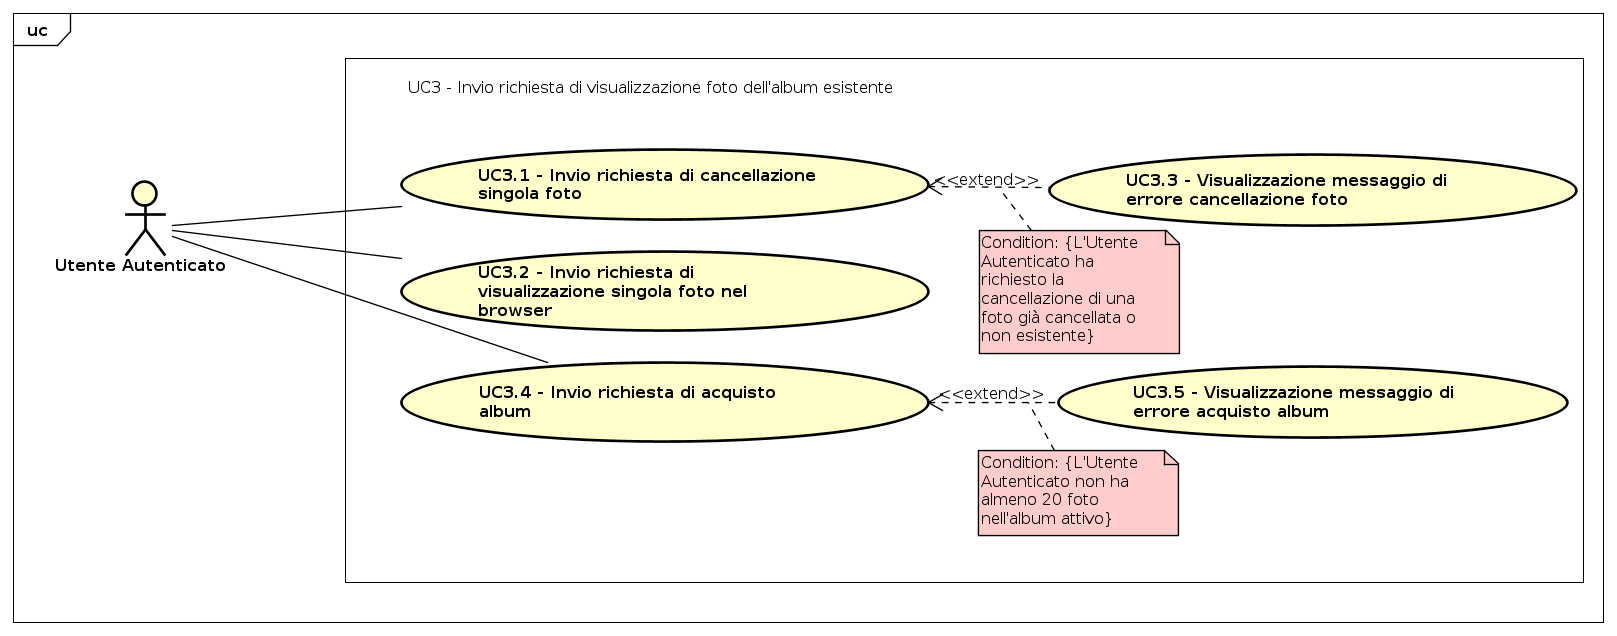
\includegraphics[scale=0.35]{useCase/UC3}
  \caption{UC3: invio richiesta di visualizzazione foto dell'album attivo}
\end{figure}


%\newpage

\subsection{UC12: visualizzazione messaggio di errore album vuoto}
\label{uc:uc12}
\hypertarget{UC12}{}

\begin{itemize}
  \item \textbf{Attori}: Utente Autenticato;
  \item \textbf{Descrizione}: questa situazione avviene quando non sono
presenti foto all'interno dell'album;
  \item \textbf{Precondizione}: l'Utente Autenticato ha richiesto la
visualizzazione dell'album vuoto;
  \item \textbf{Postcondizione}: l'Utente Autenticato ha visualizzato con
successo il messaggio di errore;
  \item \textbf{Flusso principale}:
  \begin{enumerate}
    \item L'Utente Autenticato richiede la visualizzazione dell'album senza
fotografie
  \end{enumerate}
\end{itemize}


%\newpage

\subsection{UC3.1: cancellazione singola foto}
\label{uc:uc3.1}
\hypertarget{UC3.1}{}


\begin{itemize}
  \item \textbf{Attori}: Utente Autenticato;
  \item \textbf{Descrizione}: l'Utente Autenticato richiede la cancellazione di
una foto dall'album;
  \item \textbf{Precondizione}: l'Utente Autenticato ha la lista delle foto
presenti nell'album;
  \item \textbf{Postcondizione}: l'Utente Autenticato ha rimosso con successo
una foto dall'album;
  \item \textbf{Flusso principale}:
  \begin{enumerate}
    \item L'Utente Autenticato invia la richiesta per rimuovere una foto
dall'album
  \end{enumerate}
  \item \textbf{Scenari alternativi}:
  \begin{enumerate}
    \item L'Utente Autenticato riceve un messaggio di errore nella
cancellazione della foto (\hyperlink{UC3.3}{UC3.3})
  \end{enumerate}
\end{itemize}


%\newpage

\subsection{UC3.2: visualizzazione singola foto nel browser}
\label{uc:uc3.2}
\hypertarget{UC3.2}{}

\begin{itemize}
  \item \textbf{Attori}: Utente Autenticato;
  \item \textbf{Descrizione}: l'Utente Autenticato vuole visualizzare in maniera
dettagliata e con la massima qualità disponibile una foto presente nell'album;
  \item \textbf{Precondizione}: l'Utente Autenticato ha la lista delle foto
presenti nell'album;
  \item \textbf{Postcondizione}: l'Utente Autenticato ha visualizzato con
successo una foto dall'album;
  \item \textbf{Flusso principale}:
  \begin{enumerate}
    \item L'Utente Autenticato visualizza la foto dall'album
  \end{enumerate}
\end{itemize}


%\newpage

\subsection{UC3.3: visualizzazione messaggio di errore cancellazione foto}
\label{uc:uc3.3}
\hypertarget{UC3.3}{}

\begin{itemize}
  \item \textbf{Attori}: Utente Autenticato;
  \item \textbf{Descrizione}: questo caso si verifica quando l'Utente
Autenticato ordina la cancellazione di una foto già cancellata o ordina la
cancellazione di una foto di un album non più esistente;
  \item \textbf{Precondizione}: l'Utente Autenticato ha ordinato la
cancellazione di una foto non esistente o già cancellata;
  \item \textbf{Postcondizione}: l'Utente Autenticato ha visualizzato il
messaggio di errore con successo;
  \item \textbf{Flusso principale}:
  \begin{enumerate}
    \item L'Utente Autenticato riceve un messaggio di errore nel tentativo di
cancellare una specifica foto
  \end{enumerate}
\end{itemize}


%\newpage

\subsection{UC3.4: acquisto album}
\label{uc:uc3.4}
\hypertarget{UC3.4}{}

\begin{itemize}
  \item \textbf{Attori}: Utente Autenticato;
  \item \textbf{Descrizione}: l'utente è soddisfatto dell'album creato e vuole
procederne all'acquisto;
  \item \textbf{Precondizione}: l'Utente Autenticato ha la lista delle foto
presenti nell'album e in quell'album ci sono almeno venti foto;
  \item \textbf{Postcondizione}: l'Utente Autenticato ha acquistato con
successo l'album;
  \item \textbf{Flusso principale}:
  \begin{enumerate}
    \item L'Utente Autenticato acquista l'album
  \end{enumerate}
  \item \textbf{Scenari alternativi}:
  \begin{enumerate}
    \item L'Utente Autenticato ottiene un messaggio di errore di acquisto album
(\hyperlink{UC3.5}{UC3.5})
  \end{enumerate}
\end{itemize}

%\newpage

\subsection{UC3.5: visualizzazione messaggio di errore acquisto album}
\label{uc:uc3.5}
\hypertarget{UC3.5}{}

\begin{itemize}
  \item \textbf{Attori}: Utente Autenticato;
  \item \textbf{Descrizione}: questo errore avviene quando l'Utente Autenticato
tenta di acquistare un album con meno di venti fotografie;
  \item \textbf{Precondizione}: l'Utente Autenticato ha richiesto l'acquisto
dell'album;
  \item \textbf{Postcondizione}: l'Utente Autenticato ha visualizzato il
messaggio di errore;
  \item \textbf{Flusso principale}:
  \begin{enumerate}
    \item L'Utente Autenticato riceve un messaggio di errore relativo
all'impossibilità di effettuare l'acquisto per mancanza di foto
  \end{enumerate}
\end{itemize}


%%% FINE SEZIONE USE CASE 3 %%%


%\newpage

\subsection{UC4: invio richiesta di informazioni sui costi}
\label{uc:uc4}
\hypertarget{UC4}{}

\begin{itemize}
  \item \textbf{Attori}: Utente Autenticato;
  \item \textbf{Descrizione}: permette all'Utente Autenticato di avere
informazioni riguardo ai costi degli album e ai relativi costi di spedizione;
  \item \textbf{Precondizione}: L'Utente Autenticato ha cominciato la
conversazione con il \textit{bot};
  \item \textbf{Postcondizione}: L'Utente Autenticato ha visualizzato con
successo le informazioni sui costi;
  \item \textbf{Flusso principale}:
  \begin{enumerate}
    \item L'Utente Autenticato richiede le informazioni relative ai costi
  \end{enumerate}
\end{itemize}


%\newpage

\subsection{UC5: invio comando di aiuto}
\label{uc:uc5}
\hypertarget{UC5}{}

\begin{itemize}
  \item \textbf{Attori}: Utente Autenticato;
  \item \textbf{Descrizione}: in caso l'Utente Autenticato si trovi in una
situazione di difficoltà e non sappia quale operazione intraprendere, ha la
possibilità di chiedere aiuto per ricevedere delle istruzioni su come
utilizzare PastBot;
  \item \textbf{Precondizione}: l'Utente Autenticato ha cominciato la
conversazione con il \textit{bot};
  \item \textbf{Postcondizione}: l'Utente Autenticato ha visualizzato con
successo le istruzioni sull'utilizzo di PastBot;
  \item \textbf{Flusso principale}:
  \begin{enumerate}
    \item L'Utente Autenticato richiede le informazioni sull'utilizzo di
PastBot
  \end{enumerate}
\end{itemize}


%\newpage

\subsection{UC6: invio richiesta di visualizzazione album nel sito web}
\label{uc:uc6}
\hypertarget{UC6}{}

\begin{itemize}
  \item \textbf{Attori}: Utente Autenticato;
  \item \textbf{Descrizione}: è possibile visualizzare l'album nel sito web
dell'azienda;
  \item \textbf{Precondizione}: l'Utente Autenticato ha cominciato la
conversazione con il \textit{bot};
  \item \textbf{Postcondizione}: l'Utente Autenticato viene reindirizzato al
sito della compagnia con successo;
  \item \textbf{Flusso principale}:
  \begin{enumerate}
    \item l'Utente Autenticato invia la richiesta di visualizzare l'album nel
sito della compagnia
  \end{enumerate}
\end{itemize}

%\newpage

\subsection{UC7: invio di un comando non valido}
\label{uc:uc7}
\hypertarget{UC7}{}

\begin{itemize}
  \item \textbf{Attori}: Utente Autenticato;
  \item \textbf{Descrizione}: è possibile che venga inviato un comando non
interpretabile da parte di PastBot. Questo farà mandare a PastBot un messaggio
con le istruzioni e il suo utilizzo;
  \item \textbf{Precondizione}: l'Utente Autenticato ha cominciato la
conversazione con il \textit{bot};
  \item \textbf{Postcondizione}: l'Utente Autenticato riceve con successo un
messaggio di aiuto;
  \item \textbf{Flusso principale}:
  \begin{enumerate}
    \item l'Utente Autenticato invia un comando non valido per PastBot
  \end{enumerate}
\end{itemize}


%\newpage

\subsection{UC8: invio di uno sticker}
\label{uc:uc8}
\hypertarget{UC8}{}

\begin{itemize}
  \item \textbf{Attori}: Utente Autenticato;
  \item \textbf{Descrizione}: è possibile da parte degli utenti che utilizzano
la piattaforma di messaggistica Messenger inviare anche degli \textit{stickers}
a PastBot;
  \item \textbf{Precondizione}: l'Utente Autenticato ha cominciato la
conversazione con il \textit{bot};
  \item \textbf{Postcondizione}: l'Utente Autenticato visualizza con successo
la risposta di PastBot;
  \item \textbf{Flusso principale}:
  \begin{enumerate}
    \item L'Utente Autenticato invia uno \textit{sticker}
  \end{enumerate}
\end{itemize}


%\newpage

\subsection{UC9: invio allegato}
\label{uc:uc9}
\hypertarget{UC9}{}

\begin{itemize}
  \item \textbf{Attori}: Utente Autenticato;
  \item \textbf{Descrizione}: si ha la possibilità di inviare degli allegati a
PastBot, per esempio per poter popolare il proprio album con delle immagini;
  \item \textbf{Precondizione}: l'Utente Autenticato ha cominciato la
conversazione con il \textit{bot};
  \item \textbf{Postcondizione}: l'Utente Autenticato visualizza un messaggio
di successo di salvataggio dell'allegato;
  \item \textbf{Flusso principale}:
  \begin{enumerate}
    \item L'Utente Autenticato invia un allegato a PastBot
  \end{enumerate}
  \item \textbf{Scenari alternativi}:
  \begin{enumerate}
    \item Visualizzazione messaggio di errore per tipo di allegato non valido
(\hyperlink{UC10}{UC10})
  \end{enumerate}
\end{itemize}


%\newpage

\subsection{UC10: visualizzazione messaggio di errore per tipo di allegato non
valido}
\label{uc:uc10}
\hypertarget{UC10}{}

\begin{itemize}
  \item \textbf{Attori}: Utente Autenticato;
  \item \textbf{Descrizione}: questo messaggio di errore viene visualizzato
quando viene inviato un tipo di allegato che non sia una immagine a PastBot;
  \item \textbf{Precondizione}: l'Utente Autenticato ha cominciato la
conversazione con il \textit{bot};
  \item \textbf{Postcondizione}: l'Utente Autenticato visualizza un messaggio
di errore con successo;
  \item \textbf{Flusso principale}:
  \begin{enumerate}
    \item L'Utente Autenticato invia un allegato che non è un'immagine
supportata
  \end{enumerate}
\end{itemize}


\newpage

\subsection{UC11: visualizzazione menù permanente}
\label{uc:uc11}
\hypertarget{UC11}{}

\begin{itemize}
  \item \textbf{Attori}: Utente Autenticato;
  \item \textbf{Descrizione}: l'Utente Autenticato ha accesso al menù
permanente con il quale può inviare comandi al \textit{bot} senza doverli
inserire tramite la tastiera;
  \item \textbf{Precondizione}: l'Utente Autenticato ha cominciato la
conversazione con il \textit{bot};
  \item \textbf{Postcondizione}: l'Utente Autenticato esegue le operazioni
desiderate con successo;
  \item \textbf{Flusso principale}:
  \begin{enumerate}
    \item L'Utente Autenticato può effettuare la richiesta di creazione di un
nuovo album (\hyperlink{UC11.1}{UC11.1})
    \item L'Utente Autenticato può richiedere la visualizzazione delle foto
esistenti nell'ultimo album creato (\hyperlink{UC11.2}{UC11.2})
    \item L'Utente Autenticato può richiedere le informazioni sui prezzi
(\hyperlink{UC11.3}{UC11.4})
    \item L'Utente Autenticato può richiedere la visualizzazione del messaggio
di aiuto (\hyperlink{UC11.4}{UC11.4})
  \end{enumerate}
\end{itemize}

\begin{figure}[H]
  \centering
  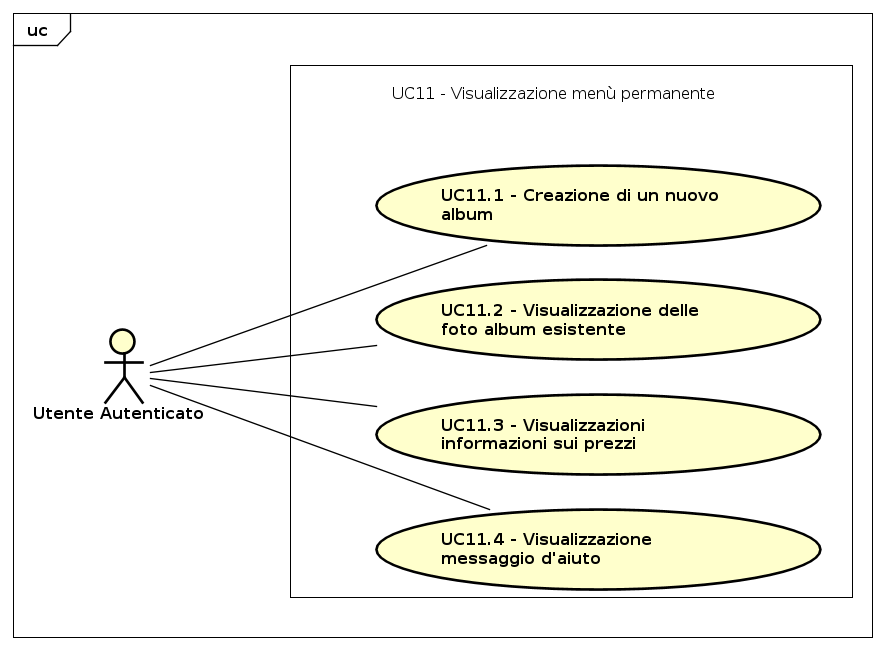
\includegraphics[scale=0.3]{useCase/UC11}
  \caption{UC11: visualizzazione menù permanente}
\end{figure}


%\newpage

\subsection{UC11.1: creazione di un nuovo album}
\label{uc:uc11.1}
\hypertarget{UC11.1}{}

\begin{itemize}
  \item \textbf{Attori}: Utente Autenticato;
  \item \textbf{Descrizione}: ciò permette all'Utente Autenticato di creare un
nuovo album semplicemente cliccando un bottone;
  \item \textbf{Precondizione}: l'Utente Autenticato ha aperto il menù
permanente;
  \item \textbf{Postcondizione}: l'Utente Autenticato ha inviato la richiesta
di creazione di un nuovo album con successo;
  \item \textbf{Flusso principale}:
  \begin{enumerate}
    \item L'Utente Autenticato richiede la creazione di un nuovo album
  \end{enumerate}
\end{itemize}


%\newpage

\subsection{UC11.2: visualizzazione delle foto dell'album esistente}
\label{uc:uc11.2}
\hypertarget{UC11.2}{}

\begin{itemize}
  \item \textbf{Attori}: Utente Autenticato;
  \item \textbf{Descrizione}: tramite questa funzionalità sarà possibile per
l'Utente Autenticato visualizzare le foto presenti nell'album in maniera
semplice;
  \item \textbf{Precondizione}: l'Utente Autenticato ha aperto il menù
permanente;
  \item \textbf{Postcondizione}: l'Utente Autenticato ha inviato la richiesta
di visualizzazione delle foto di un album esistente con successo;
  \item \textbf{Flusso principale}:
  \begin{enumerate}
    \item L'Utente Autenticato richiede la visualizzazione delle foto di un
album
  \end{enumerate}
\end{itemize}
